\documentclass[12pt, letterpaper]{article}
\usepackage[colorlinks]{hyperref}
\usepackage[utf8]{inputenc}
\usepackage{graphicx}
\usepackage{caption}
\usepackage{subcaption}
\graphicspath{ {../Log/} }

\title{Analysis Report on Inspecting MQTT}
\author{Liyao Tang - u6142160}
\date{ \today}

\begin{document}
\begin{titlepage}
	\maketitle
\end{titlepage}

\section{Analysis on Handshakes under Different QoS}

Figure \ref{fig:handshake_snap_shot} shows the required screenshots. QoS defines the handshake of the sending and receiving of one message between the sender and receiver, which both can be either broker or devices. For each QoS level, an explanation of its handshake are given as follow.
\begin{enumerate}

	\item QoS = 0
	
	The application message is delivered according to the best efforts of the underlying TCP/IP network and sender would discard the application message once sent out. 
	
	Hence, the application message will arrive at receiver at most once.
	
	\item QoS = 1
	
	After application message sent, sender waits for an acknowledgement (PUBACK or Publish Ack) to make sure the application message is received. To match PUBACK with corresponding application message, each application message at this QoS level has an ID. After PUBACK received, application message can be safely discarded.
	
	After a predefined time without returning PUBACK for the application message, sender will re-send application message with its DUP flag set, meaning this is duplicate. 
	
	Hence, the application message will arrive at receiver at least once.
	
	\item QoS = 2
	
	After application message sent, sender waits for an acknowledgement (PUBREC or Publish Received) to ensure application message is received and then responds with a further acknowledgement (PUBREL or Publish Release) to acknowledge that it knows application message is received. Afterwards, sender still needs to wait for one more acknowledgement (PUBCOMP or Publish Complete) from receiver so that sender is sure that receiver has received the PUBREL. Finally, the application message can be safely discarded.
	
	After a predefined time without the expecting message, the protocol (either sender or receiver) will retry from the last unacknowledged message.
	
	Hence, the application message will arrive at receiver exactly once.
	
\end{enumerate}

As listed above, those assisting messages that is not compulsory for application to meet its specification can transmit on QoS level 0; whereas those key messages, which may results in deviation from the specification if not received, should transmit under QoS level 1; while some important messages whose not only payload but also occurrence matter should transmit under QoS level 2 because duplicate messages are not applicable under this circumstance.

\begin{figure}
	\centering
	\begin{subfigure}[t]{0.77\textwidth}
		\centering
		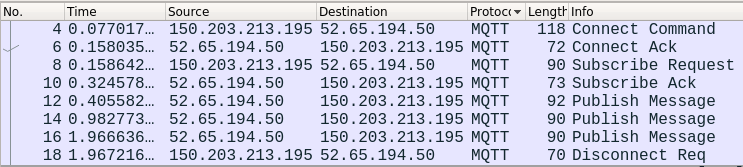
\includegraphics[width=\textwidth]{handshake-q0}
		\caption{QoS = 0}
	\end{subfigure}
	
	\begin{subfigure}[t]{0.77\textwidth}
		\centering
		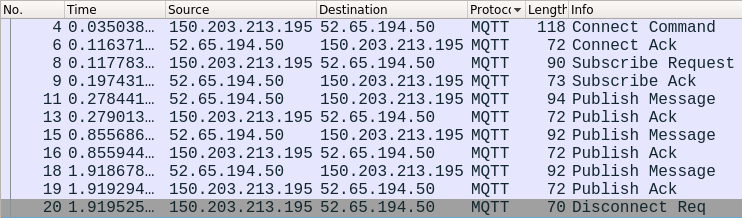
\includegraphics[width=\textwidth]{handshake-q1}
		\caption{QoS = 1}
	\end{subfigure}
	
	\begin{subfigure}[t]{0.77\textwidth}
		\centering
		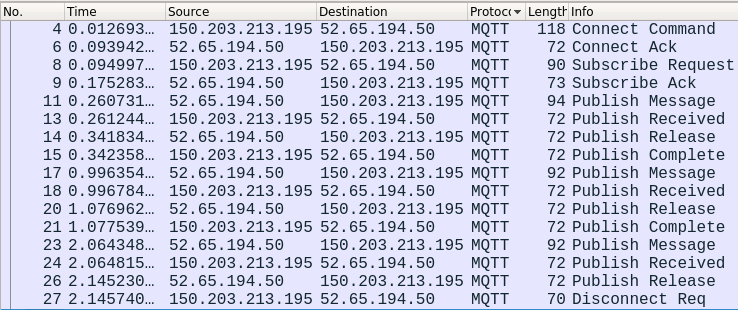
\includegraphics[width=\textwidth]{handshake-q2}
		\caption{QoS = 2}
	\end{subfigure}

	\caption{Figures of MQTT handshake under different QoS. The client disconnects the broker after receives three messages.}
	\label{fig:handshake_snap_shot}
\end{figure}


\end{document}

